%%%%%%%%%%%%%%%%%%%%%%%%%%%%%%%%%%%%%%%%%%

\chapter{Demonstration of simultaneous spin analyzer}\label{chap:ssa_2020}

%%%%%%%%%%%%%%%%%%%%%%%%%%%%%%%%%%%%%%%%%%

Measurements took place in 2020. Initial version of \acrshort{ssa} was tested.

\begin{figure}
    \centering
    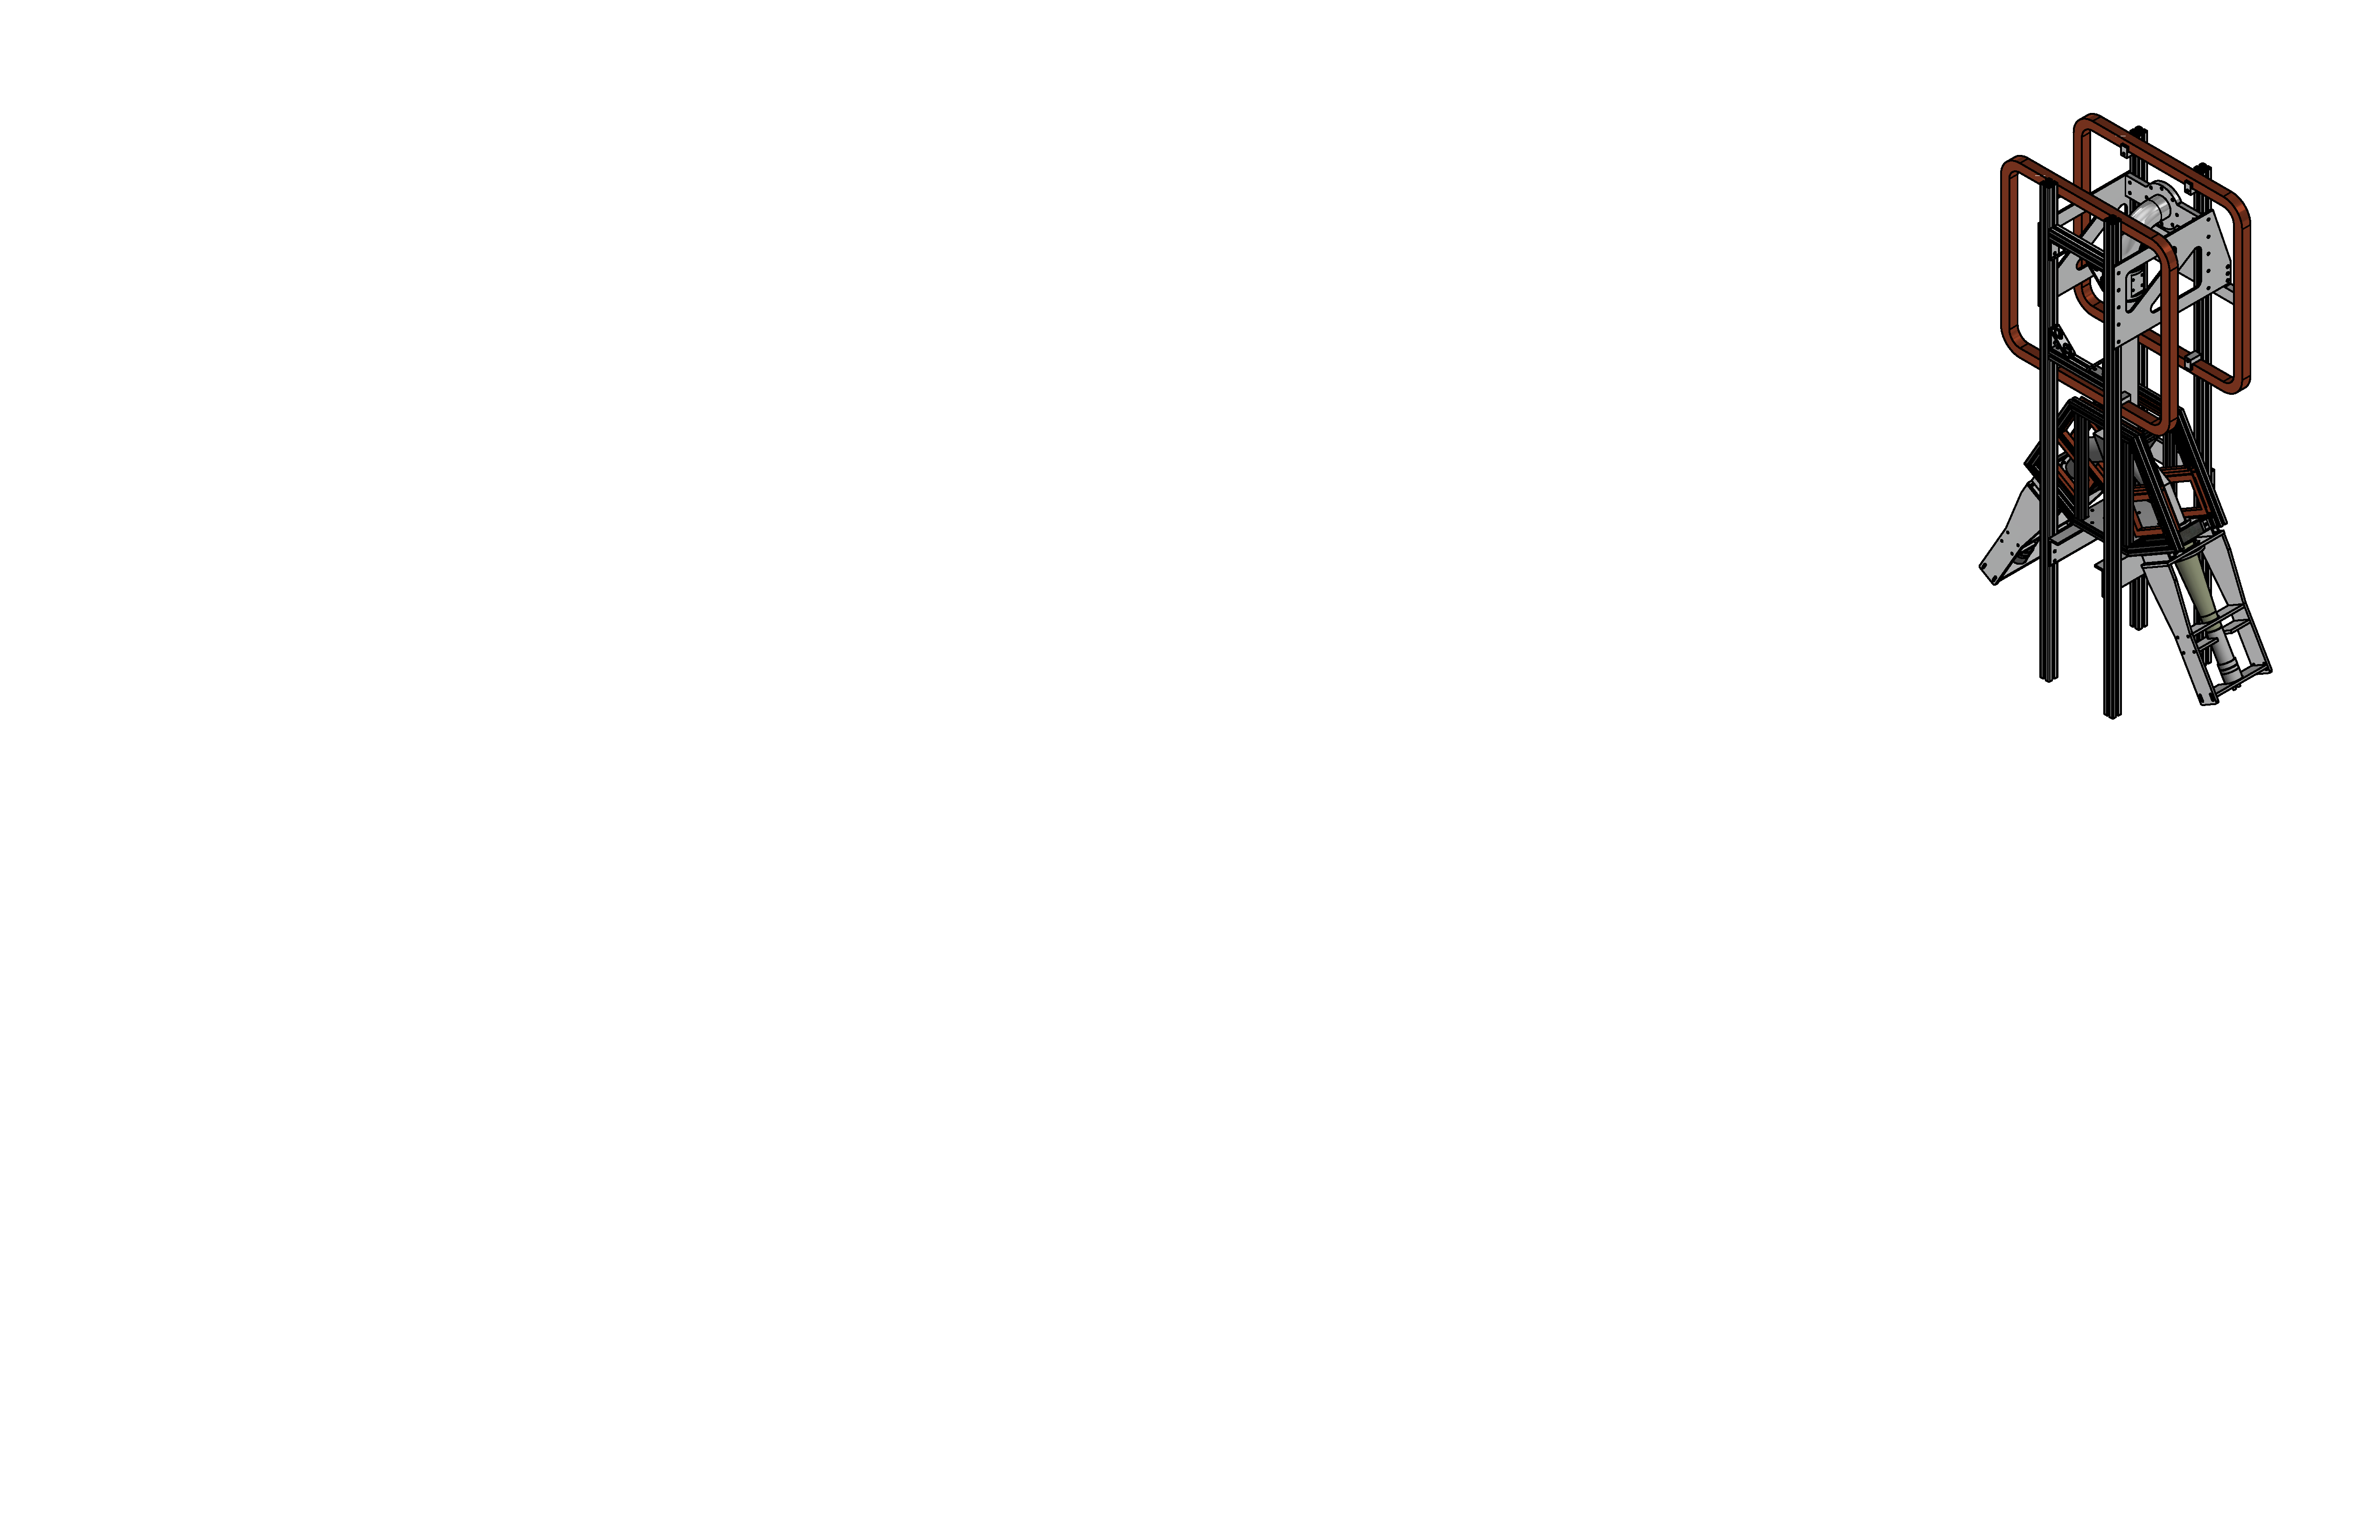
\includegraphics[height=3.1in]{figures/ssa_schematic_colorized.pdf}
    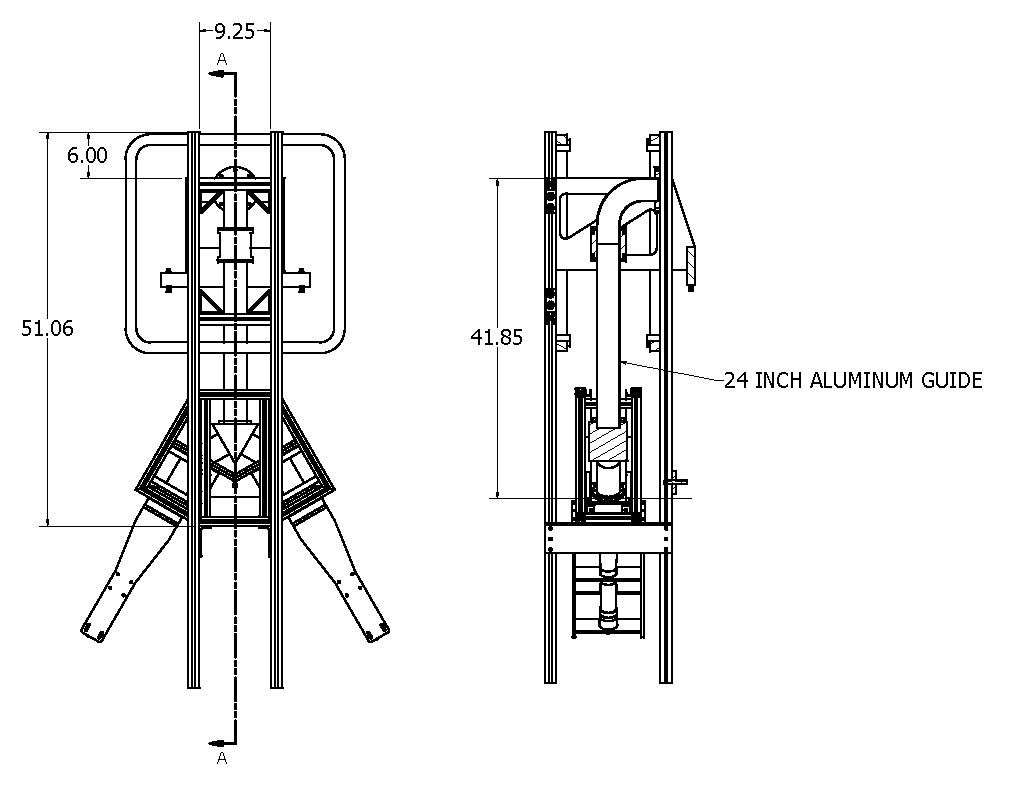
\includegraphics[height=3.5in]{figures/ssa_schematics.pdf}
    \caption
    {Schematics for first iteration of simultaneous spin analyzer, mounting frame, and associated transport coils. Courtesy of Mark Luxnat.}
    \label{fig:ssa_schematic}
\end{figure}

%%%%%%%%%%%%%%%%%%%%%%%%%%%%%%%%%%%%%%%%%%

\section{Description of apparatus}

%%%%%%%%%%%%%%%%%%%%%%%%%%%%%%%%%%%%%%%%%%

Same polarizer, \BZnS scintillator , iron yoke design. Mounted on a free switcher port. Other port had the single arm. 

%%%%%%%%%%%%%%%%%%%%%%%%%%%%%%%%%%%%%%%%%%

\section{Flow through measurement}

%%%%%%%%%%%%%%%%%%%%%%%%%%%%%%%%%%%%%%%%%%

Flow through measurement of single arm for comparison in Fig.~\ref{fig:spin_flipper_efficiency}


%%%%%%%%%%%%%%%%%%%%%%%%%%%%%%%%%%%%%%%%%%

\section{Modifications for second iteration}

%%%%%%%%%%%%%%%%%%%%%%%%%%%%%%%%%%%%%%%%%%

Wound RF coils with higher coil count and removed aluminum sleeve.

Increased guide drop with NiP coated segment

New power supply with higher amplitude. keithley 6517b

PMTs changed out for SiPMs for a better vacuum seal and to avoid potential complications of PMTs under a large magnetic field

Silicon Photomultiplier(SiPM) 4-Side Scaleable Arrays. Array C Series